\documentclass{article}
    % General document formatting
    \usepackage[margin=0.7in]{geometry}
    \usepackage[parfill]{parskip}
    \usepackage[utf8]{inputenc}
    % To add links to web pages
    \usepackage{hyperref}    
    % Related to math
    \usepackage{amsmath,amssymb,amsfonts,amsthm}
    \usepackage{mathtools}
    % We add some formats to account for our mathematical proposition    
    \newtheorem{proposition}{Proposition}
    % THE DOCUMENT BEGINS!
\begin{document}

\title{\textbf{Identification of repeated sequences in the context of DNA-barcodes}}
\author{Johannes Borgqvist}
\date{\today}
\maketitle
\tableofcontents
\listoffigures
\thispagestyle{empty}
\clearpage
\setcounter{page}{1}
\section{The number of repeated molecular bar codes could be formulated as a lottery problem}
A few days ago, my dear friend Gustav Johansson (soon to earn his PhD title) approached me with a problem from his research. He said that he wanted to know the expected number of
repititions when labelling molecules with so called molecular bar codes. However, to simplify a bit, he formulated
the problem as a lottery problem. So here comes my interpretation of how he formulated the problem:

\begin{center}
  \textsf{Imagine that you have a lottery with 1000 tickets labelled with integers from 1 to 1000. Then you conduct the following three steps: draw a lottery ticket, record its number and put the ticket back.
    Next, suppose that this procedure was repeated say 100 times meaning that you would end up with a list of a hundred integers. How many times are you expected to have repeated numbers in this list (e.g. doublettes, triplettes etc.)? Just for simplicity, let us stick with doublettes.
  What is the expected number of doublettes in this list containing 100 integers?}
  \end{center}

The aim of this document is to try to answer the above question theoretically using fundamental probability theory. Furthermore, the composition of this document is divided into three parts. Firstly, the relevant notation from probability theory is introduced, secondly the derivation of the theoretical expected value is presented and thirdly
the theoretical expected value is compared to simulations based on random number generators. 

\section{Introducing notation based on probability theory and deriving the mathematical formulation of the problem}
We begin by introducing some notation for the total number of lottery tickets and
the size of the sample drawn from this set. Drawing from the above description, let
$n\in\mathbb{N}_+$ (e.g. $n=1000$) be the number of lottery tickets and let $k\in\mathbb{N}_+$ (e.g. $k=100$) be
the length of the list or the size of the sample if you wish. Next, in order to make
the formulas as general as possible, we will introduce a variable $r\in\mathbb{N}_+$ for the number of
repeating values where $r=2$ corresponds to doublettes and $r=3$ corresponds to triplettes etc. Now, we are ready to introduce our sample space $\mathcal{S}$ corresponding to \textit{the set of all possible outcomes} \cite{devore2008probability,rice2006mathematical}. For the sake of illustrating this point, let us reduce the sample size to $k=10$. Then, one outcome of repeatedly drawing 10 values could, for example, be the list $\mathbf{l}_1$ below

\begin{equation}
\mathbf{l}_1=\begin{pmatrix}1\\10\\223\\567\\379\\909\\78\\175\\1\end{pmatrix}.
\label{eq:list}
\end{equation}
Now, the sample space $\mathcal{S}$ consists of all such lists, i.e.
\begin{equation}
\mathcal{S}\coloneqq\left\{\mathbf{l}_1,\mathbf{l}_2,\ldots,\mathbf{l}_T\right\}
\label{eq:sampleSpace}
\end{equation}
where the number of elements in this set denoted by the integer $T\in\mathbb{N}_+$. Moreover, this integer is related to the binomial coefficient $C_k$ obtained by the classical ``n choose k'' formula \cite{devore2008probability,rice2006mathematical}

\begin{equation}
C_k={n\choose k} =\dfrac{n!}{k!(n-k)!}
  \label{eq:combinations}
\end{equation}
where ``!'' corresponds to the factorial operator, e.g. $3!=3\cdot 2\cdot 1=6$. To compute the number of combinations with repititions one has to use the following variation of \eqref{eq:combinations}

\begin{equation}
C_k'={n+k-1\choose k}. 
  \label{eq:combinationsRepititions}
\end{equation}
Thus, the integer $T\in\mathbb{N}_+$ corresponding to the number of elements in $\mathcal{S}$ is given by the latter modified binomial coefficient in \eqref{eq:combinationsRepititions}, i.e. $T=C_k'$. According to \eqref{eq:combinations}, the number of lists that can be generated in the case when $n=100$ and $k=10$ is

$${100\choose 10}= 17310309456440$$
so the number of combinations is quite large already for small sample sizes.
Although we are talking about large numbers, it is still important to bare in mind that we are talking about \textit{finite} sets, and more precisely we have a finite discrete sample space $\mathcal{S}$. We will now proceed by defining a \textit{random variable} (in the context of probability theory) on this set, and let us recall that \textit{a random variable is a function $x$ on $\mathcal{S}$ which maps an outcome $\mathbf{l}_i\in\mathcal{S}$ to a real number, i.e. $x:\mathcal{S}\mapsto\mathbb{R}$} \cite{devore2008probability,rice2006mathematical}.

To this end, let $x_r:\mathcal{S}\mapsto\mathbb{N}_+$ be the random variable which assigns the number of repeated sequences of length $r$ (e.g. $r=2$ corresponds to doublettes meaning repeated double entries, $r=3$ corresponds triplettes, $r=4$ corresponds quadruplettes etc.) to a given list $\mathbf{l}_i\in\mathcal{S}$. For example, for the list $\mathbf{l}_1$ in \eqref{eq:list} on page \pageref{eq:list} we would have $x_2(\mathbf{l}_1)=1$ as there is one doublette with the value $1$. Moreover, the probability $P$ for a given list to have a certain number of doublettes determined by the random variable $x_r$ is given by

\begin{equation}
P(x_r(\mathbf{l}_i))=\dfrac{\textrm{Number of succesful outcomes}}{\textrm{Total number of outcomes}}=\dfrac{N(x_r(\mathbf{l}_i))}{T}
\label{eq:probability}
\end{equation}
and here it is appropriate to remind ourselves of the previously introduced variable $r$ corresponding to the number of repititions where, for instance, $r=2$ corresponds to doublettes. This is on account of the fact that using the variable $r$, we can define \textit{the maximum number of allowed repititions} (read doublettes, tripplettes etc.) with a given size $r$ given by the value $R$ which can be calculated using the following formula

\begin{equation}
R=\textrm{floor}\left(\dfrac{\log\left(k\right)}{\log\left(r\right)}\right)
\label{eq:repititions}
\end{equation}
where ``$\log$'' can be any logarithm and where the ``floor'' function rounds the number to the closest integer downwards (e.g. $\textrm{floor}(3.75)=3$). The above notation and equations allow us to generalise the framework, so we do not merely have to consider doublettes but in fact one can consider repititions of any higher order such as triplettes, quadruplettes etc. Now, we have arrived at a point where it is possible to define the general formula for the expected value on a discrete probability space.

The expected value, denoted $E:\mathbb{R}\mapsto\mathbb{R}$, of repeated sequences\footnote{Again, if $r=2$ we are interested in doublettes.} of size $r$ in an arbitrary list $\mathbf{l}_i$ of size $k$ drawn from a set $\mathcal{S}$ of size $n$ is given by

\begin{equation}
E[X_r]=\sum_{i=1}^{T}x_r(\mathbf{l}_i)P(x_r(\mathbf{l}_i))
\label{eq:expectedValue}
\end{equation}
where $X_r:\mathcal{S}\mapsto\mathbb{R}_+$ is a discrete random variable denoting the number of repeated sequencs of length $r$ with set of possible values in $\mathcal{S}$ and where the sum is taken over all elements in $\mathcal{S}$ \cite{devore2008probability,rice2006mathematical}. By combining the equations in \eqref{eq:combinations}, \eqref{eq:combinationsRepititions}, \eqref{eq:probability}, and \eqref{eq:expectedValue} we can now derive a theoretical value for a lower and an upper boundary value of the expected value of doublettes in a drawn list of a certain length. 


\section{An upper and a lower bound on the theoretical formula for the expected number of repetitions}
For the sake of simplicity, let us start with the case of the expected value of doublettes $r=2$ (we will be able to generalise this later on). Let us begin by considering lists of the sort presented in \eqref{eq:list} where the value $1$ is repeated once or in other words let us consider lists containing \textit{exactly} one doublette with the value 1. Also, for arguments sake, let us assume that $n=1000$ and $k=100$. Now, for all such lists there are $n-i=n-1=999$ (for an index $i=1$ corresponding to the number of doublettes) values to choose the remaining $k-r^i=k-2=98$ (\textit{unique}) elements in the list given that the entries with the value $1$ are fixed. To this end, let the index $i=1$ denote the number of repititions of a given length $r$, or the number of doublettes in the specific case $r=2$. Given this index $i$, there are exactly

$${n-i\choose k-r^i}={n-1\choose k-2}={999\choose 98}$$
lists in $\mathcal{S}$ where an entry with value $1$ is repeated once (denoted by the index $i=1$), i.e. where we have exactly one doublette with the value $1$. In total, we can keep $n={n\choose i}={n\choose 1}$ values fixed in a similar fashion, and hence the number of lists with exactly one doublette must be

$$N(x_r=i)= {n\choose i}\cdot{n-i\choose k-r^i}$$
and thus the probability to draw a list with exactly one doublette must be
$$P(x_r=i)=\dfrac{{n\choose i}\cdot{n-i\choose k-r^i}}{{n+k-1\choose k}}$$
for the index $i=1$ which is obtained by dividing the number of list with exactly one doublette by the total number of lists according to \eqref{eq:probability}. Since the number of doublettes is \textit{exactly} $1$ for these lists,
it follows that the corresponding random variables are $x_r=i=1$ meaning that the weights for all these terms in the sum in \eqref{eq:expectedValue}
is one. Thus, the part of the sum in \eqref{eq:expectedValue} which yields the expected value corresponding to lists with exactly one doublette can be summarised as follows

$$E_i=i\cdot\left(\dfrac{{n\choose i}\cdot{n-i\choose k-r^i}}{{n+k-1\choose k}}\right)$$
where the index $i=1$ means that we have exactly \textit{one} repitition of a given size $r$ (again $r=2$ in the case of doublettes). 

Next, consider the vectors where the value $1$ and $2$ are repeated once, i.e. lists where we have one doublette with the value $1$
and one doublette with the value $2$. This means that we update our index to the value ``$i\gets 2$'' if you will. For such lists $\mathbf{l}_i$, we have that our random variables satisfy $x_r(\mathbf{l}_i)=i=2$ which will be the coefficients in the sum. Using the same logic as before, there are $n-i=n-2=998$ values to choose the remaining $k-r^i=k-4=96$ (\textit{unique}) values in the list $\mathbf{l}_i$ from which means that there are exactly 
$${n-i\choose k-r^i}={n-2\choose k-4}={998\choose 96}$$
such lists in $\mathcal{S}$ where we have two doublettes with the values $1$ and $2$ respectively. Furthermore, there are ${n\choose i}={n\choose 2}$ such pairs that can be held fixed which means that there are
$$N(x_r=i)= {n\choose i}\cdot{n-i\choose k-r^i}$$
lists in $\mathcal{S}$ for the index $i=2$ where containing exactly two doublettes. According to \eqref{eq:probability}, the corresponding probability is given by dividing this number by the total number of outcomes according to

$$P(x_r=i)=\dfrac{{n\choose i}\cdot{n-i\choose k-r^i}}{{n+k-1\choose k}}.$$
Accordingly,the part of the sum in \eqref{eq:expectedValue} which corresponds to lists with exactly $i=2$ doublettes are given by
$$E_i=i\cdot\left(\dfrac{{n\choose i}\cdot{n-i\choose k-r^i}}{{n+k-1\choose k}}\right).$$
Owing to our hard work with establishing such a rigorous notation, it is now quite simple to obtain the overall expectation. The overall expectation $E_L[X_r]$ in \eqref{eq:expectedValue} is just obtained by summing all partial expectated values $E_i$ with respect to all indices $i\in\left\{1,\ldots,n\right\}$ implying that

$$E_L[X_r]=\sum_{i=1}^R E_i.$$
Consequently, the theoretically expected number of repeated entries of value $r$ is given by

\begin{equation}
  E_L[X_r]=\displaystyle\sum_{i=1}^R i\cdot\left(\dfrac{{n\choose i}\cdot{n-i\choose k-r^i}}{{n+k-1\choose k}}\right).
  \label{eq:expectedLower}
  \end{equation}
Using \eqref{eq:expectedLower}, it is possible to calculate the expected number of repeated numbers of length $r$ for a given sample of size $k$ drawn from $n$ integers. Observe that there are two importants observations to make about \eqref{eq:expectedLower}. Firstly, we sum until the number of repeated partitions $R$ in \eqref{eq:repititions} are reached. Secondly, the expected value in \eqref{eq:expectedLower} constitute a \textit{lower bound} of the actual expected value. This is due to the fact that only a limited number of repeated segments with length $r$ is counted and these are precisely the lists containing a specific number of repeated sequences of length $r$ where the remainder of the generated list $\mathbf{l}$ only contains \textit{unique} elements. This implies that numerous lists with the given number of repeated segments of length $r$ are missed since elements with longer repititions in the remainder of the list will be neglected. Let us expemplify this by considering two lists $\mathbf{l}_1$ and $\mathbf{l}_2$ respectively of length $k=10$ where we are interested in doublettes, i.e. $r=2$,

$$\mathbf{l}_1=\begin{pmatrix}1\\ 1\\ 3\\ 2\\ 5\\ 4\\7\\8\\9\\10\end{pmatrix}\;\;\textrm{and}\;\;\mathbf{l}_2=\begin{pmatrix}1\\ 1\\ 3\\ 2\\ 5\\ 4\\9\\9\\9\\10\end{pmatrix}.$$
Now, in \eqref{eq:expectedLower} only $\mathbf{l}_1$ will be counted as it contains one doublette while the remainder of the list contains unique elements. However, $\mathbf{l}_2$ will be missed despite the fact that it also contains one doublette and this is on account of the triplette of the value $9$ at the end of the list. To account for these missing values, it is important to account for repititions in the remainder of the list and this can be done by replacing the binomial coefficient $C_k$ in \eqref{eq:combinations} with the adapted binomial coefficient $C_k'$ in \eqref{eq:combinationsRepititions}. 

Using this modification of \eqref{eq:expectedLower}, it is possible to obtain an \textit{upper}\footnote{Note that the subscripts ``$L$'' and ``$U$'' in, for example, $E_L[X_r]$ correspond to the lower and upper bound respectively.} \textit{bound} $E_U[X_r]$ 


\begin{equation}
  E_U[X_r]=\displaystyle\sum_{i=1}^R i\cdot\left(\dfrac{{n\choose i}\cdot{(n-i)+(k-r^i)-1\choose k-r^i}}{{n+k-1\choose k}}\right).
  \label{eq:expectedUpper}
  \end{equation}
Note here that we do account for repititions in the remainder of the list. In other words, if we are interested in the number of doublettes, we do account for triplettes, quadruplettes etc. in the remainder of the list. However, we also account for doublettes in the remainder of the list which implies that multiple doublettes are \textit{counted twice}! Accordingly, too many values are included in this formula which means that $E_U[X_r]$ in \eqref{eq:expectedUpper} constitutes an upper bound of the actual expected value. In other words, if the actual expected value is denoted$E[X_r]$ the follwing holds

$$E_L[X_r]< E[X_r]< E_U[X_r].$$
All the above arguments are summarised in the following proposition. 


\begin{proposition}
  Let $n,k,r\in\mathbb{N}_+$ be three positive integers such that $n>k>r>1$ holds. Assume that one element is drawn from the set $\{1,2,3,\ldots,n\}$, that the value of this element is saved in a list $\mathbf{l}$ and that the element then is put back into this set. Moreover, assume that this procedure is repeated $k$ times such that the generated list $\mathbf{l}$ contains $k$ elements after the sampling procedure, and denote the set of all possible lists generated by this procedure by $\mathcal{S}\coloneqq\left\{\mathbf{l}_1,\mathbf{l}_2,\ldots,\mathbf{l}_T\right\}$. Let $r$ be the length of a repeated sequences in a given list $\mathbf{l}\in\mathcal{S}$, where $r=2$ corresponds to doublettes and $r=3$ corresponds to triplettes etc. Also, let $x_r:\mathcal{S}\mapsto\mathbb{N}_+$ be a random variable which counts the number of sequences of length $r$ in a given list $\mathbf{l}\in\mathcal{S}$. Then, the expected number of repeated sequences of length $r$ in an arbitrary list $\mathbf{l}$ generated by the above procedure denoted by $E[X_r]$ where $E[X_r]:\mathbb{R}\mapsto\mathbb{R}$ satisfies the following bounds
$$E_L[X_r]< E[X_r]< E_U[X_r]\Longleftrightarrow E[X_r]\in\left(E_L[X_r],E_U[X_r]\right)$$
  where $X_r:\mathcal{S}\mapsto\mathbb{R}_+$ is a stochastic random variable on $\mathcal{S}$ indicating the number of repeated sequences of length $r$. The lower bound $E_L$ is given by \eqref{eq:expectedLower} on page \pageref{eq:expectedLower} and the upper bound $E_U$ is given by \eqref{eq:expectedUpper} on page \pageref{eq:expectedUpper}.
  \label{prop:expectation}
\end{proposition}
Also, it is very interesting to check the validity of this formula which is done next by comparing the results of simulations based on random number generators with the theoretical result in Proposition \ref{prop:expectation}.


\section{Simulations reveal that the usefulness of theoretical upper and lower boundary values on the expected value is limited to small sample sizes $k$}
To test the validity of the of the theoretical results, the findings were compared to the output of simulations. To this end, lists of length $k$ where generated using a random number generator and then the number of repeated segments in the generated list was calculated. As random numbers are involved in the simulation algorithm, this procedure was repeated ``num\_of\_repeats'' times. The parameters that were fixed for the set of experiments were the following:

$$n=4^{12},\;r=2\;\textrm{and}\;\textrm{num\_of\_repeats}=1000.$$
The result from conducting this procedure once is a list of ``num\_of\_repeats'' elements, where each individual element corresponds to the number of repeated segments of length $r$ in a generated list. Given this framework, the sample size $k$ is varied in order to see its effect on the number of repeated segments. Moreover, the corresponding theoretical values are calculated for the given $(n,k,r)$-triplets. The results from these simulations show that the theoretical bounds $E_{L}$ and $E_U$ in Proposition \ref{prop:expectation} can only be useful for small sample sizes (more precisely for values $k<6000$). As can be seen in the results, we have that the upper limit blows up while the lower limit rapidly goes to zero which in equations could be expressed as follows:

$$\underset{k\rightarrow\infty}{\lim}E_L=0\;\mathrm{and}\;\underset{k\rightarrow\infty}{\lim}E_U=\infty.$$
Note that these bounds are only useful as long as the lower bound is \textit{strictly} greater than zero and the upper bound is \textit{strictly} smaller than infinity since it is then possible to predict the range of possible values for the actual expected number of repeated segments of length $r$. In practice these values should also be as close as possible meaning that $E_L$ should be as large as possible and $E_U$ should be as small as possible. Thus, it is clear from the simulations (Fig \ref{fig:simulations}c-d) that these bounds can only be used for smaller sample sizes $k$ which we will come back to. The reason why the limits formulated above hold is due to the fact that we get a combinatorial explosion in the binomial coefficients in the nominators and denominators in \eqref{eq:expectedLower} and \eqref{eq:expectedUpper}. More precisely, in the case of $E_L$ the denominator goes quicker to infinity than the nominator as $k$ goes to infinity which explains why the lower limit tends to zero for large sample sizes. Intuitively, this is due to the fact that all the combinations that are neglected in the nominator (remember that we neglected all repetitions in the remainder of the vector) goes to infinity when $k$ blows up.

In the case of the upper boundary value $E_U$, the nominator in \eqref{eq:expectedUpper} goes to infinity faster than the denominator and that is why this value tends to infinity when the sample size $k$ goes to infinity. As was stated in the beginning of this document, pretty small numbers of $n$ and $k$ yields large binomial coefficients $C_k$ and $C_k'$ which explains the very rapid rate with which the two boundary values $E_L$ and $E_U$ tend to $0$ and $\infty$ respectively (Fig \ref{fig:simulations}(c) and \ref{fig:simulations}(d)).

Thus, for larger sample sizes $k$ one has to resort to simulations (Fig \ref{fig:simulations}(a) and \ref{fig:simulations}(b)). From a computational point of view, the generation of random numbers is quite a costly operation and accordingly the run time for conducting ``num\_of\_repeats'' repitions increases proportionally with the sample size $k$. Consequently, it is of interest to speed up the computation time of the algorithm at hand for large sample sizes $k$. 
\begin{figure}[htbp!]
  \begin{center}
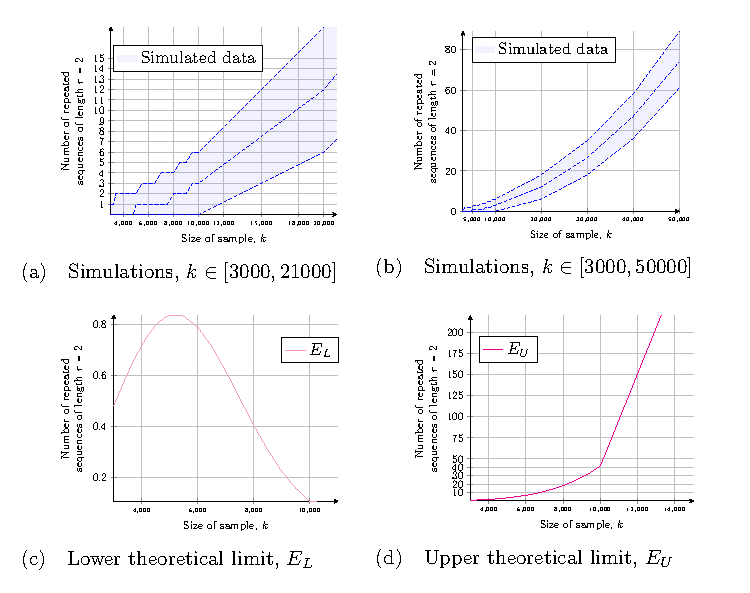
\includegraphics[width=\textwidth]{../Figures/Fig1/Fig1.pdf}
\caption[\textbf{Simulated data and the theoretical boundaries of the expected value plotted against the sample size $k$}]{\textbf{Simulated data and the theoretical boundaries of the expected value plotted against the sample size $k$}. The samples visualised in the sub figures correspond to lists with $k$ integers generated from the set $\{1,2,\ldots,n\}$ with $n=4^{12}$. In the simulations, the number of repeated sequences with length $r=2$ (i.e. doublettes) have been counted which is displayed on the y-axes (sub figures (a) and (b)) as a function of the sample size $k$. The simulations have been repeated 1000 times as the simulations are stochastic since random numbers are generated. In the sub figures (a) and (b), the 5\%, 50\% and 90\%-quantiles of the generated data sets are depicted in order to visualise the spread in the simulations. Also, the lower boundary value of the expected value $E_L$ in \eqref{eq:expectedLower} is depicted as a function of the sample size $k$ (sub figure (c)) as well as the corresponding upper boundary value $E_U$ in \eqref{eq:expectedUpper} (sub figure (d)).}
\label{fig:simulations}
  \end{center}
  \end{figure}

\section{A marginal speed up of the implemented simulation algorithm was achieved by means of CPU-parallelisation}
The solution algorithm was implemented so that the code was parallelised using multiple CPUs. The idea behind the parallelisation is simple. As the same procedure (involving the generation of $k$ random numbers and then counting the number of repeated sequences of length $r$) is repeated multiple times (or specifically ``num\_of\_repeats''=1000 times), it should be faster to conduct a set of these repitions in parallel (i.e. simultaneously) as oppose to conducting them linearly ``one at a time'' in a serial fashion. Using this logic, the more parallelisation the better, as the more operations that are conducted in parallel the faster the computations should be finished. However, there is a prize to pay for parallelising in practice (on either CPUs or GPUs) and this prize is directly proportional to the computational cost of transferring memory between the various processes involved in the parallelised execution of the script. Hence, it is usually quite costly to transfer variables stored in memory \textit{to} the various processing units initially before the calculations are done and then it is also costly to transfer the resulting data \textit{back} to the main process. It can in fact be the case that this memory transfer is so costly that parallelisation slows down the application and given this background it is perhaps no surprise that high performance computating using parallelisation is usually very hard almost considered as an art-form. The methodology for assessing whether an implemented parallelisation is succesful or not is to benchmark the code, i.e. to measure the run time of the script with different levels of parallelisations. 

To deduce whether the implemented script could be rendered more efficient or not, the run time was investigated as a funtion of the number of CPUs implemented. Specifically, the previously described algorithm with $(n,r)=(4^{12},2)$ and ``$\textrm{num\_of\_repeats}=1000$'' was benchmarked five values of k, namely $k\in\left\{10000,20000,30000,40000,50000\right\}$. In order to obtain data sets of the execution times of the scripts, the solution algorithm was repeated $30$ times, and on these data sets the $5\%$-,$50\%$- and $95\%$- quantiles were plotted as functions of these $k$-values. The results (Fig \ref{fig:HPC}) show that the implemented levels of parallelisation (3 and 5 CPUs respectively) do not enhance the efficiency of the script in a meaningful way. Thus,in order to achieve a faster implementation this naive implementation has to be extended, and the main key in decreasing the runtime lies in increasing the efficiency in transferring the generated lists between the main process and the respective CPUs. Perhaps if one increases the number of repititions stored in the variable ``num\_of\_repeats'' perhaps one can see a more substantial improvements in the performance of the script as more random numbers are required implying that the script could benefit more from parallelisation.

If one whishes to improve the code, it is just a matter of downloading the repositry at \url{github}

\begin{figure}[htbp!]
  \begin{center}
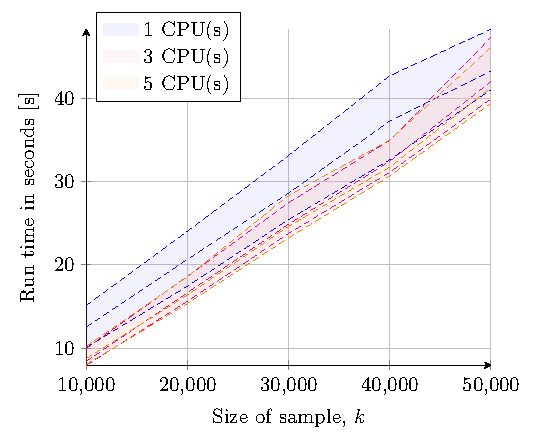
\includegraphics[width=\textwidth]{../Figures/Fig2/Fig2.pdf}
\caption[\textbf{Run time of the script plotted against the sample size $k$}]{\textbf{Run time of the script plotted against the sample size $k$}. The samples visualised in the sub figures correspond to lists with $k$ integers generated from the set $\{1,2,\ldots,n\}$ with $n=4^{12}$. In the simulations, the number of repeated sequences with length $r=2$ (i.e. doublettes) have been counted as a function of the sample size $k$. The simulations have been repeated 1000 times as the simulations are stochastic since random numbers are generated, and it is the execution time in seconds of conducting these 1000 cycles that is displayed on the y-axis. To get some data of the execution times, these cycles have been repeated 30 times. Again, the 5\%, 50\% and 95\%-quantiles are displayed in the figure, where the effect of CPU-parallelisation is investigated. The three cases investigated are: 1 CPU (the blue curve), 3 CPUs (the magenta curve) and 5 CPUs (the orange curve). }
\label{fig:HPC}
  \end{center}
  \end{figure}


\clearpage
\bibliographystyle{plain}
\bibliography{molecular}

\end{document}
